\documentclass{beamer}
\usepackage[finnish]{babel}
\usepackage[T1]{fontenc}
\usepackage[utf8]{inputenc}
\usetheme{Warsaw}
\title[Data-assimilaatio kitkamallissa]{Data-assimilaatio kitkamallissa}
\author{Tom Gustafsson}
\date{5. syyskuuta 2012}
\begin{document}

\begin{frame}
\titlepage
\end{frame}

\begin{frame}{Ongelma}

\begin{itemize}
\item Lähtökohtana: Onnistuuko huonosti tunnettujen parametrien ennustaminen elastisesta kitkamallista \emph{data-assimilaation} tarjoamien keinojen avulla?
\end{itemize}

\begin{figure}
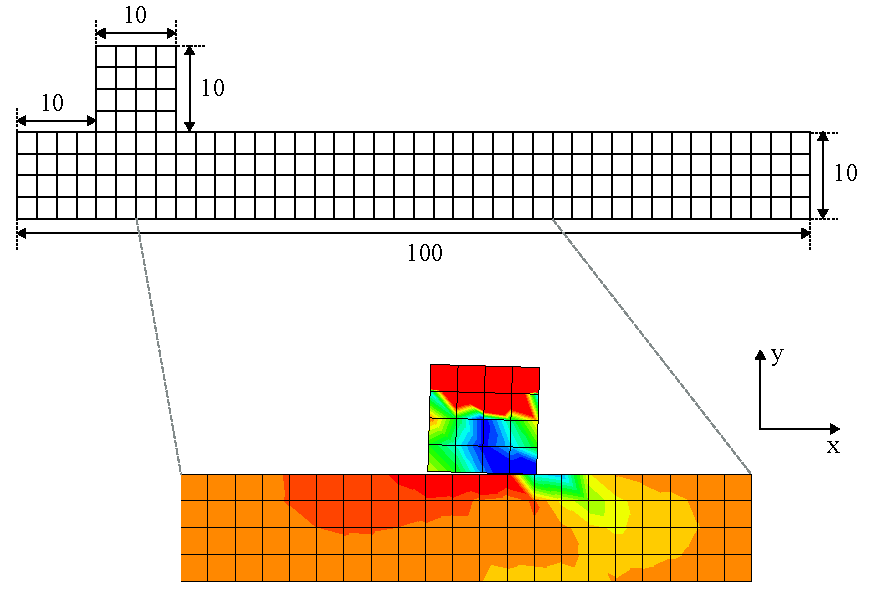
\includegraphics[width=8cm]{fretting_mesh.pdf}
\end{figure}

\end{frame}

\begin{frame}{Malli, 2D}

\begin{itemize}
\item Alkutila: Painin, laatta
\item Reunaehdot
\end{itemize}

\begin{figure}
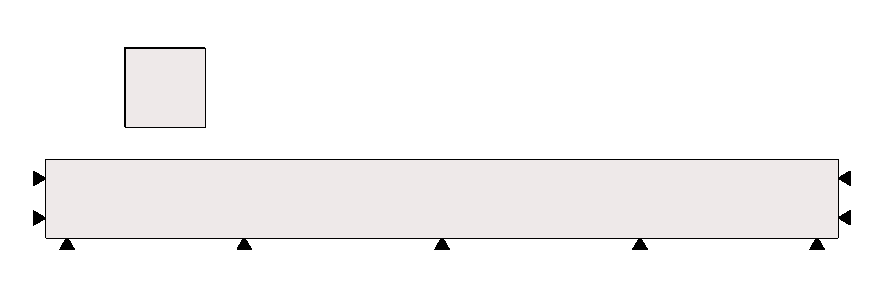
\includegraphics[width=10cm]{fretting_geom.pdf}
\end{figure}

\begin{itemize}
\item Abaqus/Standard 6.12-1, simulaatiot CSC:n koneella
\end{itemize}

\end{frame}

\begin{frame}{Simulaation vaiheet}

\begin{itemize}
\item Vaihe 1: 5 kN voima
\end{itemize}

\begin{figure}
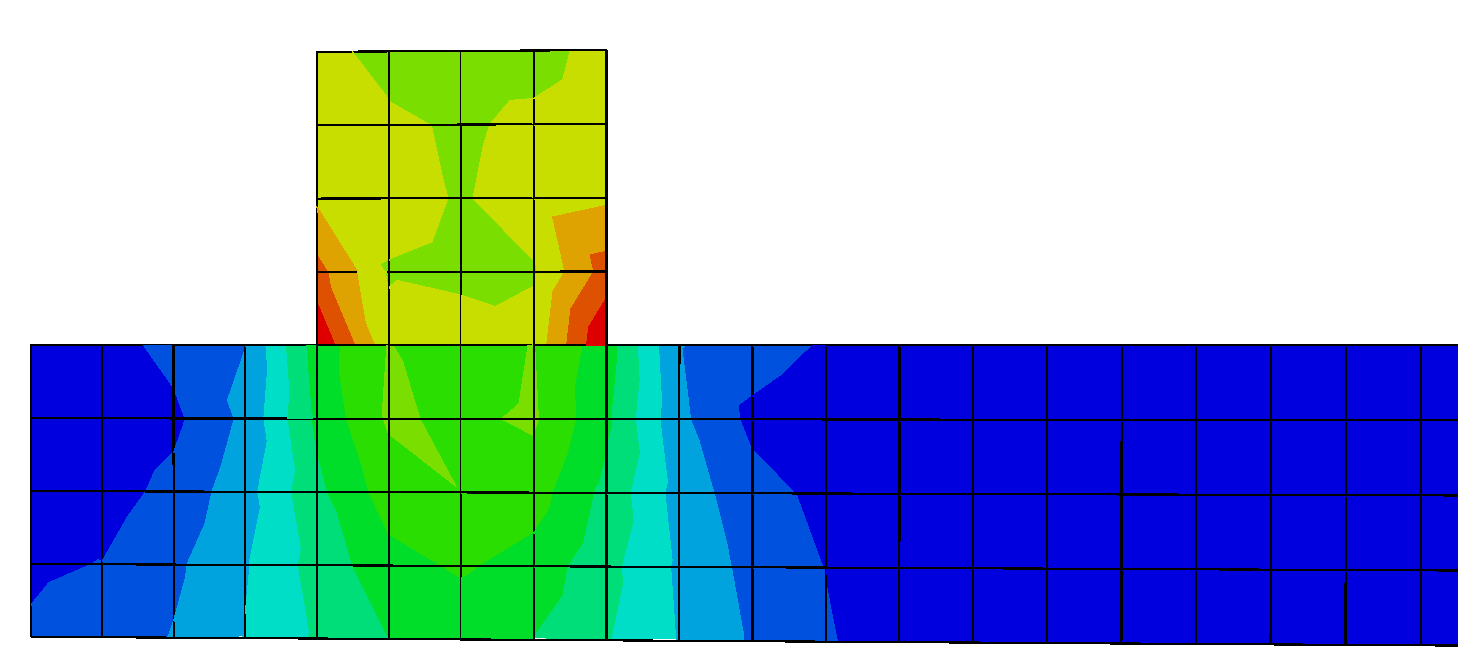
\includegraphics[width=9cm]{mises.pdf}
\end{figure}

\begin{itemize}
\item Vaihe 2: Yläreunan siirto 70 cm oikealle
\end{itemize}

\end{frame}

\begin{frame}{Simulaation vaiheet: Yläreunan siirtymä}

\begin{itemize}
\item Siirto reunaehdolla, ns. "hidas siirtymä"
\end{itemize}

\begin{figure}
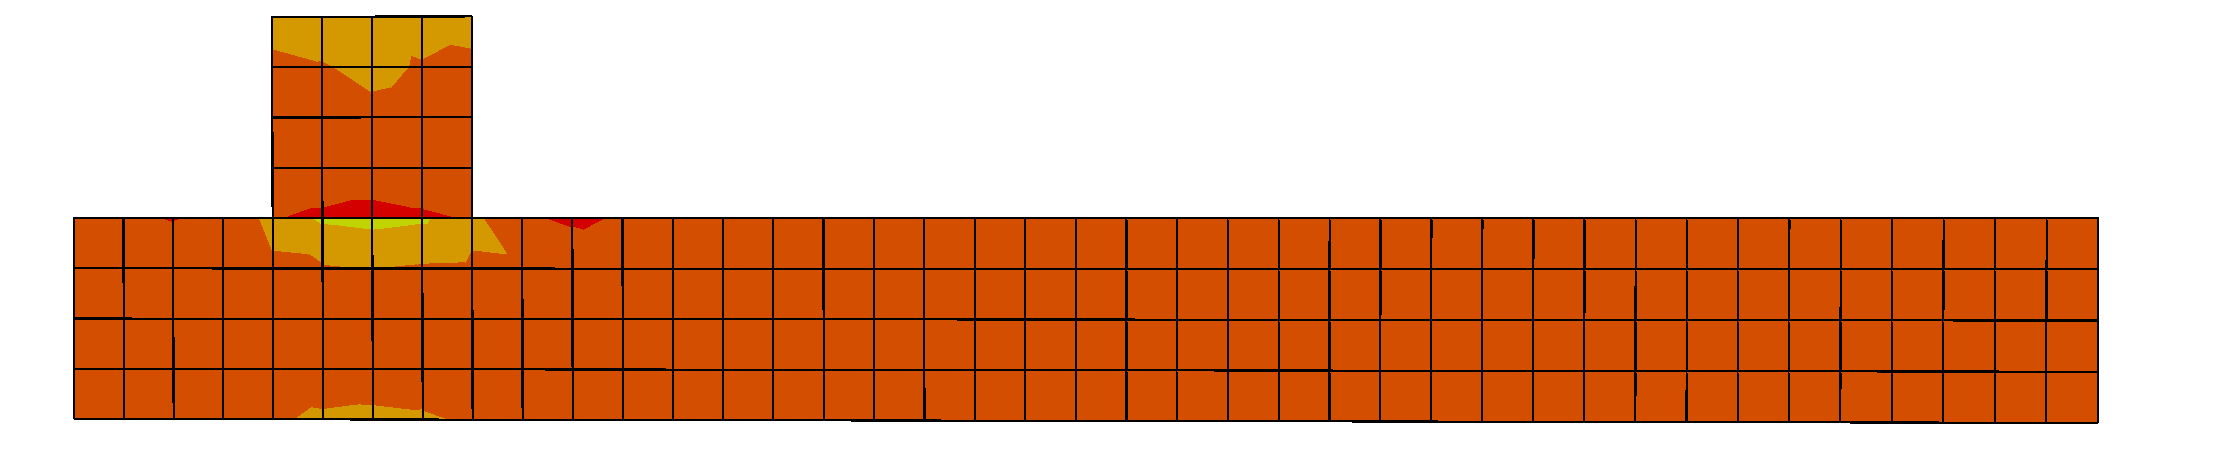
\includegraphics[width=10cm]{anim1.pdf}\\
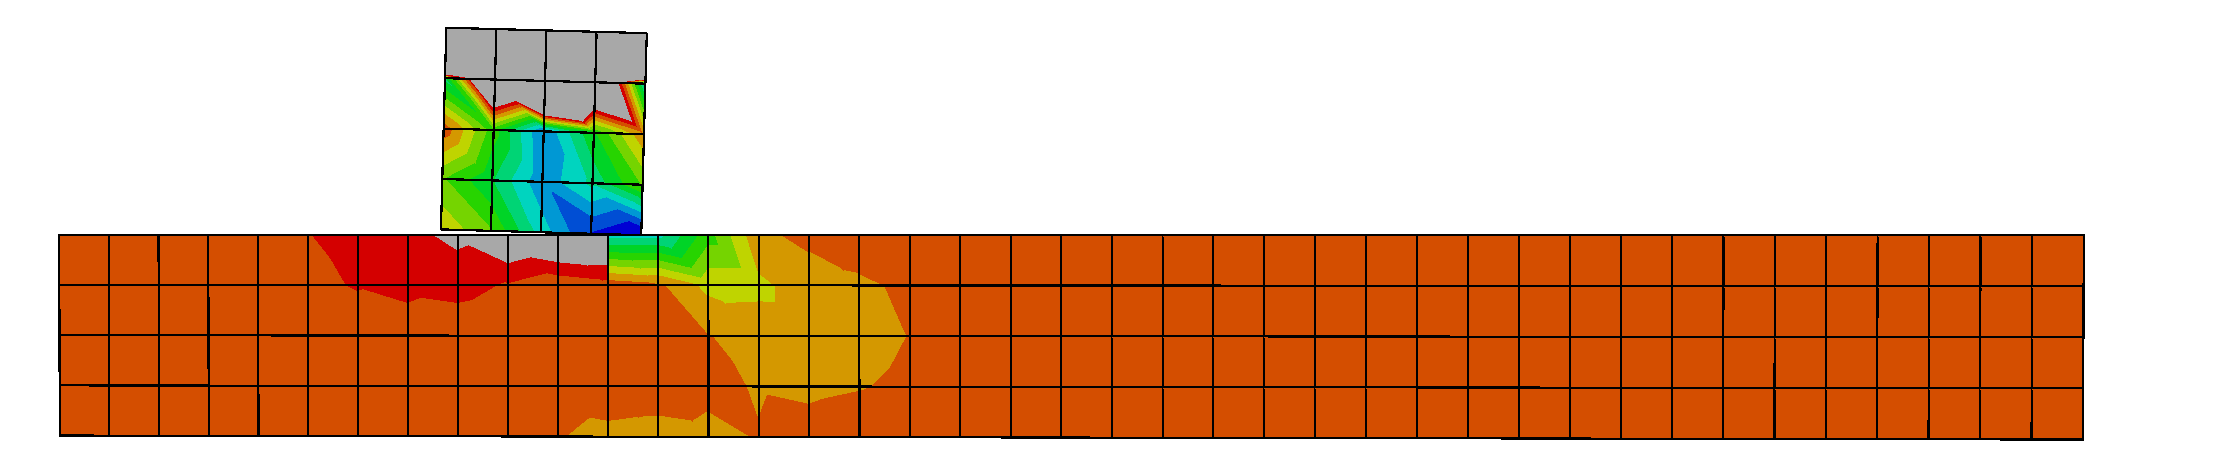
\includegraphics[width=10cm]{anim2.pdf}
\end{figure}

\end{frame}

\begin{frame}{Simulaation vaiheet: Yläreunan siirtymä 2}

\begin{figure}
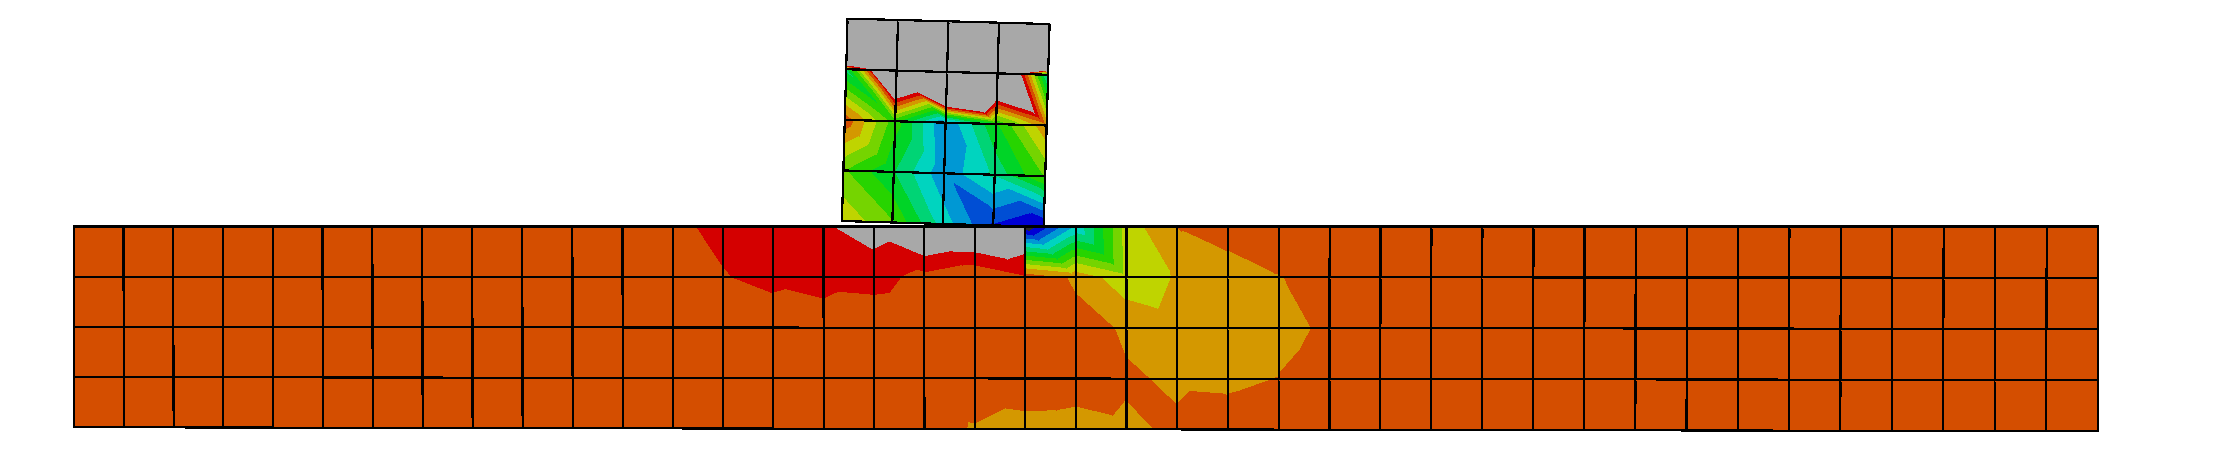
\includegraphics[width=10cm]{anim3.pdf}\\
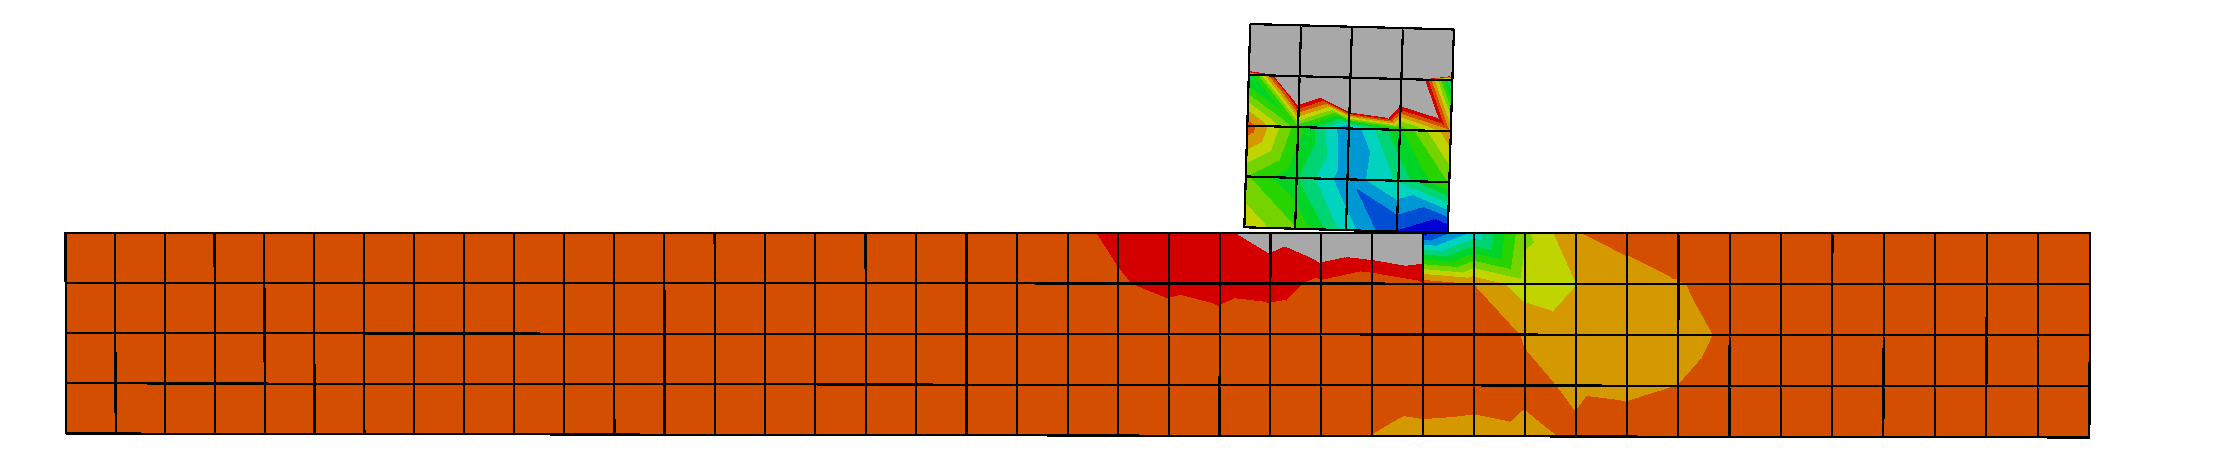
\includegraphics[width=10cm]{anim4.pdf}\\
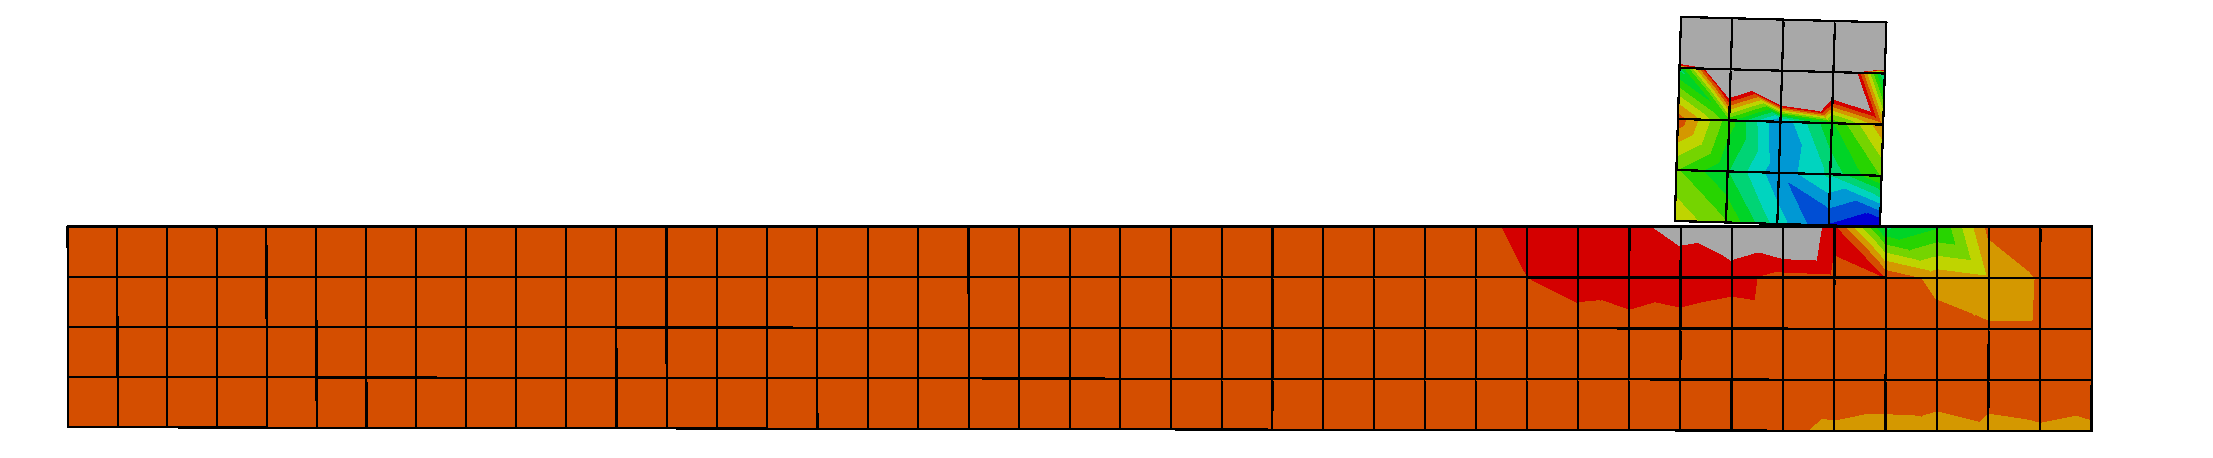
\includegraphics[width=10cm]{anim5.pdf}
\end{figure}

\end{frame}

\begin{frame}{Inversio-ongelma}

\begin{itemize}
\item Pyritään estimoimaan kitkakerroin $\mu$
\item \emph{A priori} -tietona $x$-suuntaiset jännitykset mittapisteissä\\($\sim$ venymäliuskamittaus)
\end{itemize}

\begin{figure}
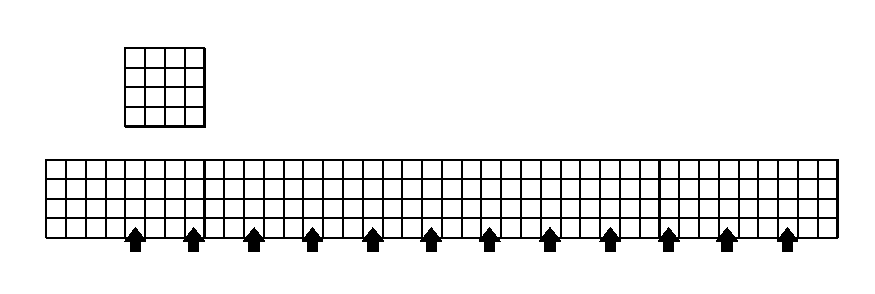
\includegraphics[width=10cm]{fretting_geom_meas.pdf}
\end{figure}

\begin{itemize}
\item Mittadata synteettistä
\end{itemize}

\end{frame}

\begin{frame}{Synteettisen mittadatan generointi}

\begin{itemize}
\item Minimoidaan inversiorikosta $\rightarrow$ mittadata tiheämmästä verkosta
\end{itemize}

\begin{figure}
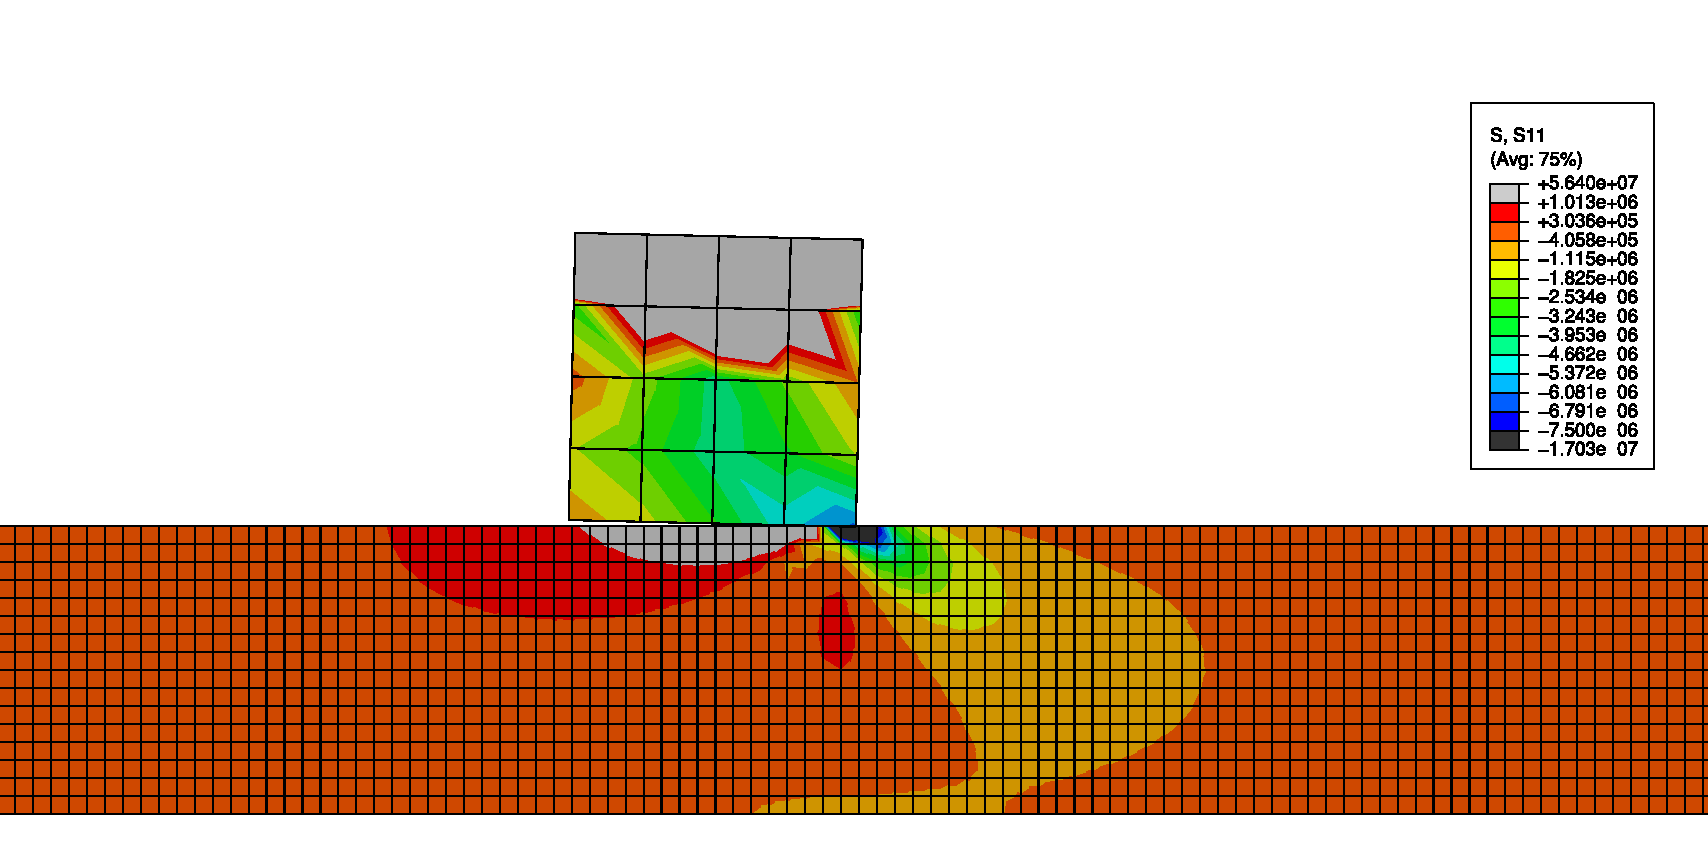
\includegraphics[width=10cm]{finer_mesh.pdf}
\end{figure}

\begin{itemize}
\item Miten verrata tiheämmän ja harvemman verkon antamia jännityksiä?
\end{itemize}

\end{frame}

\begin{frame}{Synteettisen mittadatan generointi 2}

\begin{figure}
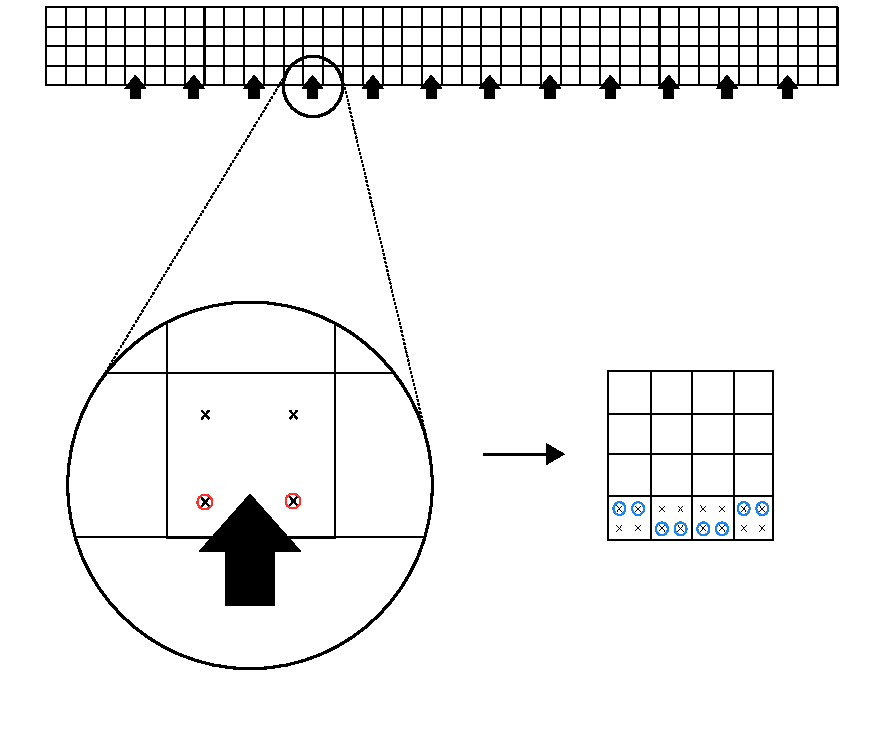
\includegraphics[width=10cm]{fretting_meas_tarkempi.pdf}
\end{figure}

\end{frame}

\begin{frame}{Ongelman yhteenveto}

\begin{itemize}
\item Estimoitava suure: Kitkakerroin $\mu=0{,}5$
\item \emph{A priori} -tieto: $x$-suuntaiset jännitykset mittapisteissä
\item Menetelmät: \emph{Data-assimilaatio}
\end{itemize}

\end{frame}

\begin{frame}{Data-assimilaatio}

\begin{itemize}
\item Pohjimmiltaan havaintojen ja mallin tuotaman informaation yhteensulauttamista
\item Perinteisiä sovelluskohteita: Säähavaintomallit, valtamerimallit
\item Data-assimilaation menetelmiä
\begin{itemize}
\item 3DVar, 4DVar
\item Kalman Filter, Extended-, Ensemble-, ...
\item ...
\end{itemize}
\item Tässä työssä \emph{Ensemble Smoother}, eli ES
\item Perustuu samaan ideaan kuin \emph{Ensemble Kalman Filter}, eli EnKF
\end{itemize}

\end{frame}

\begin{frame}{Data-assimilaatio, yleistä}

\begin{itemize}
\item Systeemin (todellinen) tila $\boldsymbol{\psi}^t \in \mathbb{R}^N$
\item Mittaus $\boldsymbol{d} \in \mathbb{R}^M$
\begin{itemize}
\item Ei tarkka
\item Suhde tilaan $\boldsymbol{d} = \mathbf{M}\boldsymbol{\psi}^t+\boldsymbol{\epsilon}$
\item Mittamatriisi $\mathbf{M} \in \mathbb{R}^{M \times N}$
\item Virhe $\boldsymbol{\epsilon} \sim \mathcal{N}_M(0,\boldsymbol{\Sigma})$
\item Kovarianssimatriisi $\boldsymbol{\Sigma} \in \mathbb{R}^{M \times M}$
\end{itemize}
\item Estimoitu tila $\boldsymbol{\psi}^f \in \mathbb{R}^N$
\begin{itemize}
\item Aluksi esim. mittauksien perusteella
\end{itemize}
\end{itemize}

\end{frame}

\begin{frame}{Data-assimilaatio, esimerkki}

$N=M=2,~\mathbf{M} = \mathbf{I},~\boldsymbol{\Sigma} = \sigma\mathbf{I}$

\begin{figure}
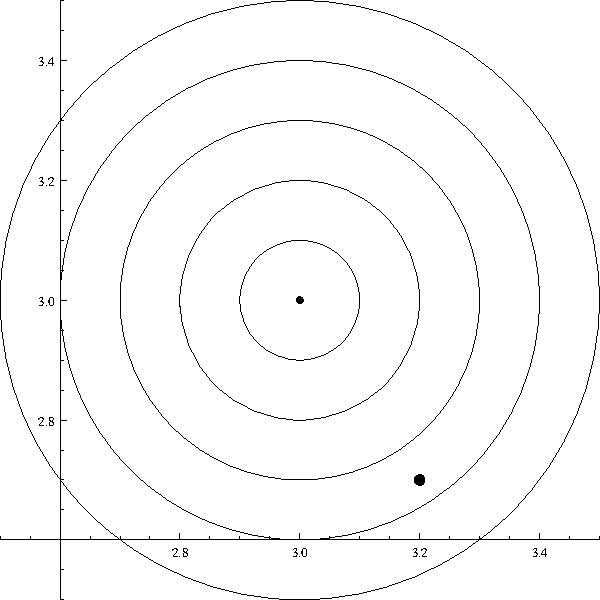
\includegraphics[width=6cm]{enkf1.pdf}
\end{figure}

\end{frame}

\begin{frame}{Data-assimilaatio, yleistä 2}

\begin{itemize}
\item Todellinen tila $\boldsymbol{\psi}^t$ muuttuu ajan kuluessa
\item Malli estimaatin aikakehityksestä:
\[
\boldsymbol{\psi}^f_{t+\Delta t} = \boldsymbol{\psi}^f_t + \int_{t}^{t+\Delta t} \! \boldsymbol{G}(\boldsymbol{\psi}^f_t,t) \, \mathrm{d}t
\]
\begin{itemize}
\item Malli epätäydellinen, eli estimaatin virhe kasvaa aikakehitettäessä
\end{itemize}
\end{itemize}

\end{frame}

\begin{frame}{Data-assimilaatio, esimerkki 2}

\begin{figure}
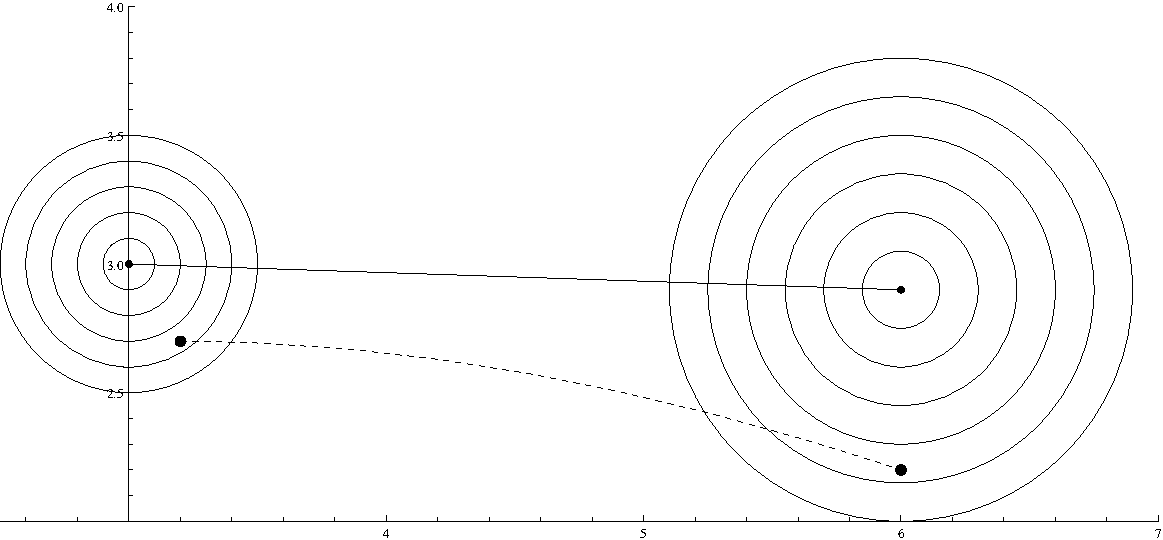
\includegraphics[width=11cm]{enkf2.pdf}
\end{figure}

\end{frame}

\begin{frame}{Data-assimilaatio, yleistä 3}

\begin{itemize}
\item Tulkitaan normaalijakauma todennäköisyystiheysfunktiona $f(\boldsymbol{\psi},t)$
\item Tällöin $f$:n aikakehitystä kuvaa \emph{Fokker-Planck -yhtälö}
\[
\frac{\partial f}{\partial t} + \sum_{i=1}^N \frac{\partial \left ( G_i f \right )}{\partial \psi_i} = \frac{1}{2} \sum_{i=1}^N \sum_{j=1}^N \frac{\partial^2 \left ( Q_{ij} f \right )}{\partial \psi_i \partial \psi_j}
\]
\item \emph{Hurja}, mutta ei niin hurja miltä näyttää (sij. $\mathbf{G} = \mathbf{0}$ ja $\mathbf{Q} = \mathbf{I}$) 
\item Yleinen tapaus ei ratkea analyyttisesti $\rightarrow$ EnKF
\end{itemize}

\end{frame}

\begin{frame}{Ensemble Kalman Filter}

\begin{itemize}
\item Idea: Otetaan $n$-kappaletta realisaatioita alkutilan normaalijakaumasta
\item Aikakehitetään näin saadun \emph{kokoelman} jokaista tilaa erikseen operaattorin $\boldsymbol{G}$ avulla
\item Etu: Estimaatin kovarianssimatriisia ei tarvitse aikakehittää (lineaarisessa $\mathcal{O}(N)$, epälineaarisessa $\mathcal{O}(N^k)$, jossa $k$ käytettävän Taylor-approksimaation aste), koska sitä voidaan approksimoida lausekkeella
\[
\boldsymbol{\Sigma} \approx \frac{1}{n-1} \sum_{i=1}^n \left( \boldsymbol{\psi}^f - \overline{\boldsymbol{\psi}^f} \right) \left(\boldsymbol{\psi}^f - \overline{\boldsymbol{\psi}^f}  \right)^\mathrm{T}
\]
\end{itemize}

\end{frame}

\end{document}
